\clearpage

\section{绪论}

\subsection{研究背景及意义}
研究生生活是一段充满智慧和探索的旅程。在这个阶段,学生们接触到更深层次的学术内容,面对更具挑战性的问题,并在学术界展开独立研究。研究生院的学术氛围让学生们有机会深入研究他们感兴趣的领域,与导师和同行们共同探讨和解决复杂的问题。

除了学术挑战,研究生生活也涵盖了更广泛的社交和职业发展。学生们与来自不同背景和领域的同学共同学习,建立起深厚的人际关系。同时,与导师的交流和合作为学生们提供了更广泛的职业发展机会,帮助他们在未来的职业生涯中更好地发展。

在研究生院,学生们有机会参与各种学术和社会活动,拓展他们的视野。这包括学术研讨会、专题讲座、学术合作项目等。通过这些活动,他们能够更全面地了解自己的专业领域,并与其他研究者建立联系。

%图片 pdf格式 测试
如图\ref{fig:w-xxx}所示

 \begin{figure}[h]
    \centering
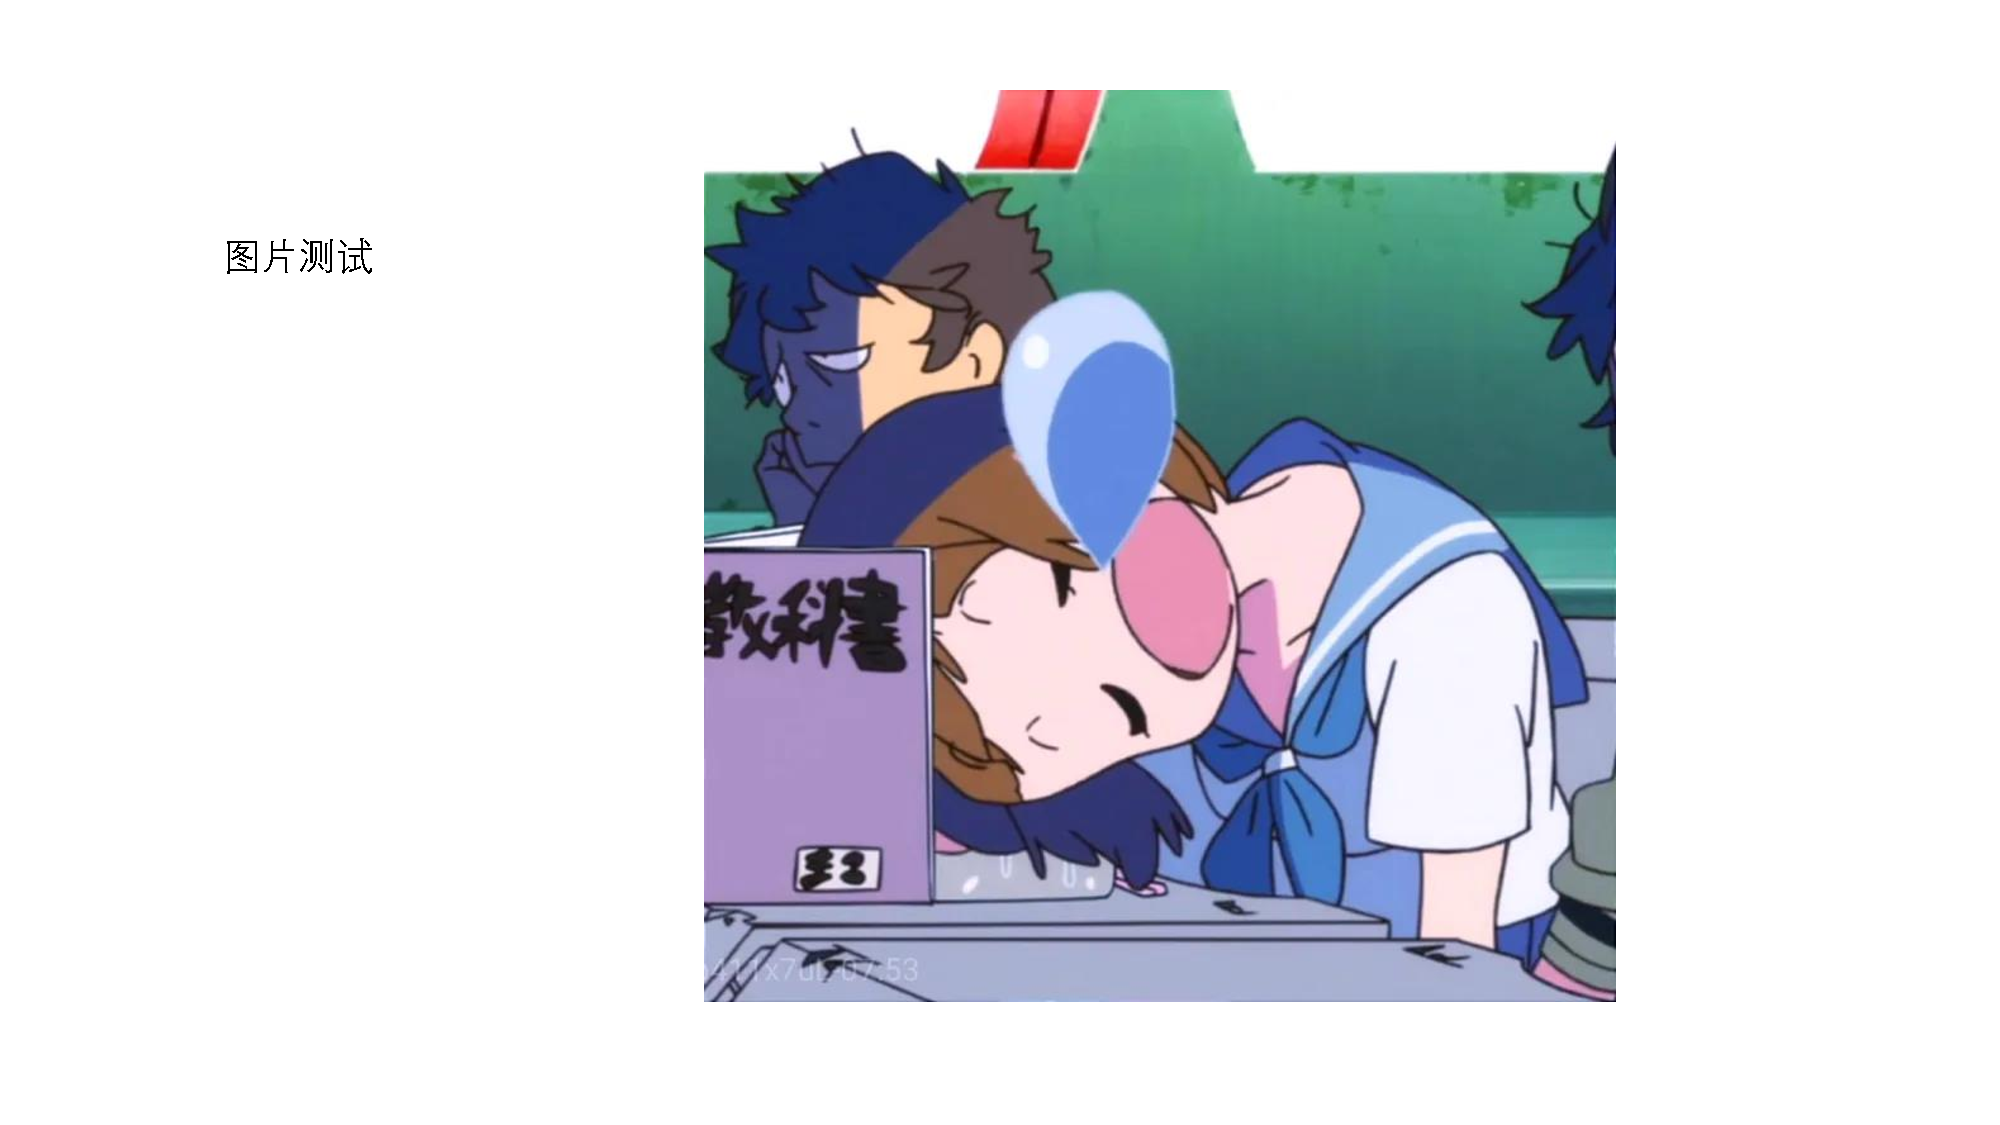
\includegraphics[width=0.8\textwidth]{figure/cp1/xxx.pdf}
     \caption{11111}  
     \label{fig:w-xxx}
 \end{figure}


如表\ref{tab:xxx}所示

% 表格测试 input插入
\begin{table*}[t]
  \centering
  \renewcommand\arraystretch{1.4}
  \caption{评估结果}
    %\resizebox{0.\textwidth}{!}{
    \begin{tabular}{l@{\hspace{4em}}c@{\hspace{4em}}c@{\hspace{4em}}c}
    \toprule
    模型 & F1 & F2 & F3  \\
    \midrule
AE & xx	 & 0.111 &	0.111 
   \\
VAE &\textbf{0.222} &	0.312 &	0.44 
 \\
    \bottomrule
    \end{tabular}%
    %}
  \label{tab:xxx}%
\end{table*}%










\subsection{研究背景及意义}
研究生生活是一段充满智慧和探索的旅程。在这个阶段,学生们接触到更深层次的学术内容,面对更具挑战性的问题,并在学术界展开独立研究。研究生院的学术氛围让学生们有机会深入研究他们感兴趣的领域,与导师和同行们共同探讨和解决复杂的问题。

除了学术挑战,研究生生活也涵盖了更广泛的社交和职业发展。学生们与来自不同背景和领域的同学共同学习,建立起深厚的人际关系。同时,与导师的交流和合作为学生们提供了更广泛的职业发展机会,帮助他们在未来的职业生涯中更好地发展。

在研究生院,学生们有机会参与各种学术和社会活动,拓展他们的视野。这包括学术研讨会、专题讲座、学术合作项目等。通过这些活动,他们能够更全面地了解自己的专业领域,并与其他研究者建立联系。